\subsubsection*{Die Elektronen}
Was nach der Ionisation mit den Elektronen geschieht, hängt von der angelegten Spannung ab. Es können die nachfolgenden Bereiche, die in Abbildung \ref{fig:DependenceVoltage} dargestellt sind, unterschieden werden.
\begin{itemize}
	\item[\textbf{I}] Ist die Spannung klein, reicht die Beschleunigung des elektrischen Felds nicht aus, um die Elektronen bis zur Anode zu bringen. Die meisten rekombinieren vorher mit den Atomrümpfen. Mit ansteigender Spannung sinkt die Rekombinationswahrscheinlichkeit schnell.ab.
	\item[\textbf{II}] Irgendwann ist die Spannung so groß, dass quasi alle Elektronen den Draht erreichen. Dann ist der zwischen Anode und Kathode fließende Strom proportional zu Energie und Intensität der Strahlung. In diesem Bereich kann man das Rohr auch als Ionisationskammer bezeichnen.
	\item[\textbf{III}] Die Elektronen werden auf dem Weg zum Draht immer stärker beschleunigt. Es gibt einen Spannungswert, ab dem ihre Energie groß genug ist, um ihrerseits wieder Atome durch Stöße zu ionisieren (Stoßionisation). Die Zahl der Ionisationen steigt lawinenartig an, man spricht hierbei von einer Townsend-Lawine. Die Ladungsmenge $Q = n\cdot e$, die pro einfallendem Strahlungsteilchen am Draht ankommt, ist nun ausreichend groß, um einen messbaren Stromimpuls zu verursachen. Da $Q$ und somit auch der Strompuls nach wie vor proportional zur Energie (und Intensität) der Strahlung ist, spricht man von einem Proportionalzählrohr.
	\item[\textbf{IV}] Die Spannung ist schließlich so groß, dass die Energie der Elektronen ausreicht, um durch inelastisches Stoßen die Atome anzuregen, die deshalb UV-Photonen emittieren. Die Photonen haben genug Energie, um Atome zu ionisieren. Da sie allerdings elektrisch neutral sind können sie sich auch senkrecht zum elektrischen Feld bewegen. Die Ionisationslawinen finden nun nicht mehr nur lokal, sondern im gesamten Volumen des Zylinders statt. Die am Draht ankommende Ladung $Q$ ist jetzt nicht nur noch proportional zur Intensität, nicht mehr zur Energie der Strahlung. Da der durch $Q$ verursachte Strom so groß ist, dass er leicht detektiert werden kann, ist dieser Bereich gut für die Intensitätsmessung von Strahlung geeignet. Hier ist auch der eigentliche Arbeitsbereich des Geiger-Müller-Zählrohrs.
	\item[\textbf{V}] 
\end{itemize}
\begin{figure}[h!]
	\centering
	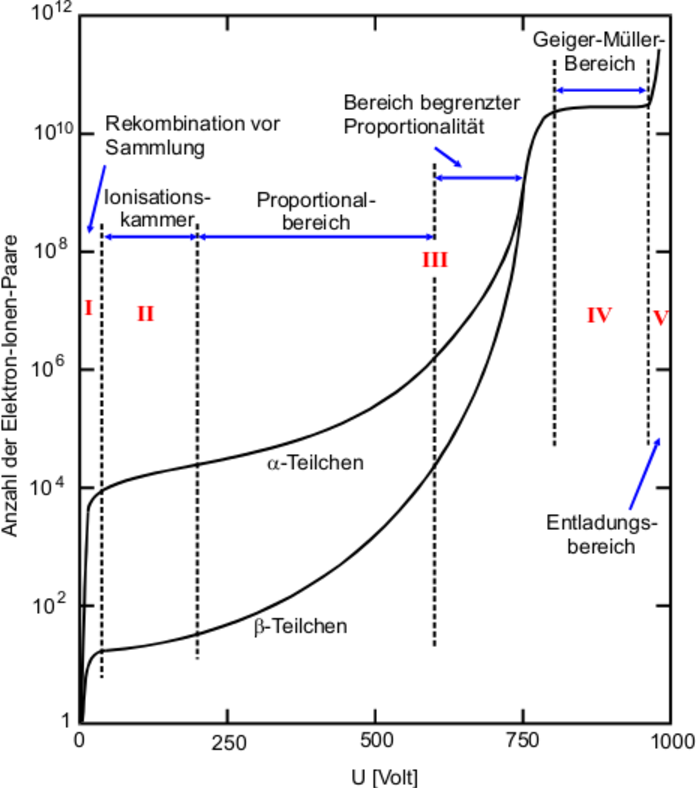
\includegraphics[width=0.6\textwidth]{Spannungsabhangigkeit.pdf}
	\caption{Anzahl der durch Ionisation frei gewordene Elektronen in Abhängigkeit von der angelegten Spannung}
	\label{fig:DependenceVoltage}
\end{figure}
